
\newcommand{\NbasesV}{\textit{N}}
\newcommand{\Nbases}{7}
\newcommand{\Nml}{7}
\newcommand{\NmlT}{5}
\newcommand{\NmlA}{2}
\newcommand{\Ncb}{4}
\newcommand{\MML}{método multirrótulo}
\newcommand{\MMLs}{métodos multirrótulo}
\newcommand{\MRLM}{Recursive Dependent Binary Relevance}
\newcommand{\MRLMa}{RDBR}

\chapter{Introdução}
\begin{verbatim}
 -Falar um pouco sobre aprendizado de máquina.
 -Falar sobre Classificação multiclasse
 -Apresentar Classificação multirrótulo e falar como é mais tenso que a multiclasse, dar exemplos etc.
 -Falar um pouco do estado da arte da Classificacao multirrotulo.
 
\end{verbatim}



\section{Motivações}
% A análise dos métodos multirrótulo traz os seguintes benefícios:
O melhor entendimento do funcionamento dos métodos multirrótulo permite:
\begin{itemize}
 \item descobrir atributos destes que se alterados, aproveitados
 e/ou combinados podem acarretar na criação de novos métodos e/ou na melhora dos existentes.
 \item prever, com uma certa taxa de erro, seus desempenhos, o que facilita o uso mais inteligente dos métodos
 sem precisar utilizar muito esforço computacional devido a testes.
 \item reforçar ou contrariar as conclusões já estabelecidas dos métodos, uma vez que a maioria delas são 
 baseadas em testes experimentais.
\end{itemize}

\section{Objetivos}
O objetivo geral deste trabalho é analisar e comparar métodos multirrótulos distintos e 
desenvolver um novo algoritmo de classificação multirrótulo.
Mais formalmente, a análise deve implicar em conclusões matemáticas ou estatísticas sobre o desempenho dos métodos multirrótulo.
O Objetivo geral pode ser detalhado nos seguintes objetivos específicos:
\begin{itemize}
 \item Comparação estatística e análise crítica dos métodos multirrótulos;
 \item Elaboração de um algoritmo de um novo método multirrótulo.
 \item Implementação dos métodos multirrótulos em uma biblioteca que integra técnicas de reconhecimento de padrões.
\end{itemize}


% \section{Contribuições}
\section{Estrutura do Trabalho}

\chapter{Classificação multirrótulo}

\section{Enunciado do problema}
\begin{verbatim}
ESBOÇO:
-Definição formal.
-um classificador multirrótulo mapeia do espaço de características
para um vetor de valores reais entre 0 e 1 
de tamanho igual ao número de rótulos.
-falar da complexidade do problema
-falar sobre lidar o problema como probabilidade condicional dado o rótulo e etc...
    P(l_1 | x,l_2)
\end{verbatim}



\section{Avaliação de Desempenho}
\begin{verbatim}
-Apresentar matematicamente o que pode indicar correlação entre rótulos e outras coisas
conforme o artigo: "Bayes Optimal Multilabel Classification via Probabilistic Classifier Chains".
-Falar que é diferente do multiclasse
\end{verbatim}
\subsection{Métricas}
\label{sec:metrics}
\subsubsection{Accuracy}
\subsubsection{Hamming-Loss}
\subsubsection{Subset Accuracy}
\subsubsection{Ranking Loss}
\subsection{Modelo de Avaliação}
\label{sec:modelav}

\begin{verbatim}
Falar do Holdout,Cross-validation estratificado.
Falar sobre bases separadas de treino,teste e validação.
\end{verbatim}

\chapter{Métodos Multirrótulos}
\section{Transformação do Problema}
\subsection{Relevância Binária - BR}
\ref{sec:br}
\subsection{Classifier Chain}
\subsection{Ensemble of Classifier Chain}
\subsection{Probabilistic Classifier Chain}
\subsection{LEAD}
\subsection{Dependent Binary Relevance - DBR}
\label{sec:dbr}
\subsection{MAIS MÉTODOS...}

\section{Adaptação de classificadores}
\subsection{ML-KNN}
\subsection{Rede Neural Artificial}
\subsection{C4.5 multirrótulo}
\subsection{CRankSVM}
\subsection{MAIS...}


\chapter{Recursive Dependent Binary Relevance - RDBR}
A proposta de \MRLM~(\MRLMa)~é fundamentada no \MML~\textit{dependent binary relevance} (DBR) \cite{dbr2014}, que é explicado
na seção \ref{sec:dbr}. Assim como o DBR e o CC, o \MRLMa~é um método baseado na transformação do problema que dividem o problema
multirrótulo em vários problemas classificação binária. Todos eles exploram a correlação entre os rótulos por meio da adição de
características especiais que representam os rótulos reais ou estimativas dos rótulos reais ao espaço de características original. 
Mas, diferentemente dos outros, o \MRLMa~adiciona uma inteligência na adição dessas características especiais na fase de predição do método.
A forma de como isso é feito bem como o funcionamento completo do algoritmo de classificação e a fundamentação teórica
do \MRLMa~são detalhados na seção \ref{sec:mrlm_algo}. 
A seção \ref{sec:mrlm_analise} analisa o funcionamento e o desempenho do \MRLMa~de forma prática, por meio de experimentos.


\section{Algoritmo de \MRLM~-~\MRLMa}
\label{sec:mrlm_algo}
Como foi dito anteriormente, o \MRLM~é baseado no DBR. 
% Ambos se baseiam na expansão do espaço de características
% com características que representam a estimativas dos rótulos como forma de explorar
% a correlação entre rótulos. Isso é feito usando a predição do BR no espaço de características original.
% Ou seja, 
Ambos dependem da hipótese de que as estimativas dos rótulos em $Y$ por um classificador multirrótulo $c_0$
são boas características para aprimorar as estimativas dos mesmos rótulos por um novo classificador $c_1$
e que quanto melhor forem as estimativas dos rótulos por $c_0$, melhores são as de $c_1$. Nesse caso, podemos dizer
que o classificador $c_0$ é usado para "alimentar" o classificador $c_1$.
E ainda ambos usam o BR como classificador multirrótulo base, que servirá para realizar as primeiras estimativas dos 
rótulos.

No entanto, o \MRLMa, ao invés de usar apenas o classificador base $c_0$ para "alimentar" $c_1$, como o DBR,
ele usa o próprio $c_1$ para se "alimentar", ou seja, há realimentação pelo próprio classificador.
A idéia é que cada vez que $c_1$ se realimente, melhores ficam suas estimativas uma vez que ele será baseado
em estimativas melhores de rótulos do que anteriormente. 
A alimentação é a propagação das 
estimativas dos rótulos de um classificador multirrótulo para o espaço de características expandido de um outro, ou o mesmo,
classificador multirrótulo. O funcionamento do algoritmo serão formalmente detalhados nas seções seguintes.

Formalmente, a estrutura do \MRLMa~é organizado da seguinte forma:
\begin{itemize}
%   \item Assim como o DBR, é composto de dois classificadores multirrotulo, o primeiro, $c_0$, é um BR
%   e o segundo, $c_1$, é um BR ligeiramente modificado, que chamaremos de $BR^*$.
  \item Assim como o DBR, é composto de um BR e um classificador multirrótulo, $c_0$ e $c_1$,
  cada um composto de $l$ classificadores binários.
  \item O $c_0$ trabalha dentro do espaço de características original do problema, de nome $X$,
  e $c_1$ trabalha dentro de um novo espaço de características do problema, de nome $X_e$ e
   definido como $X_e=X \times \{0,1\}^{l}$. Assim, $c_0$ e $c_1$ são
  representados pelas seguintes funções:
  \begin{equation}
  \begin{split}
   & c_0 : X \rightarrow \{0,1\}^l \\
   & c_1 : X_e \rightarrow \{0,1\}^l
   \end{split}
  \end{equation}
  \item Os $l$ classificadores binários $c_1^1,c_1^2...,c_1^l$ que compoêm $c_1$ não trabalham no mesmo
  espaço de características, contudo,
  trabalham com uma dimensão reduzida, em $X \times \{0,1\}^{l-1}$. Digamos que $(x,y)$ seja uma instância de $X_e$
  onde $x \in X$ e $y \in {\{0,1\}}^l$, então cada instância 
  do classificador binário $c_1^i$ tem $|x|+l-1$ características e é definido como sendo $(x,y_1,...,y_{i-1},y_{i+1},...,y_{l})$.

  
%   e o resultado da classificação multirrotulo de $c_1$ é construido da seguinte forma:
%   $c_0(x,y)=(c_1^1(x,y_2$
%   \item O método contém duas funções $t_0$ e $t_1$ que mapeiam espaços de características:
%    \begin{equation}
%  \begin{split}
%     & t_0 : X \rightarrow X_e \\
%     & t_1 : X_e \rightarrow X_e \\
%     & t_0(x)=(c_0(x)) | x \in X \\
%     & t_1(x,y)=(c_1(x,y)) | x \in X,  y \in [0,1]^{l}
% %   h_i : \mathbb{R}^l \rightarrow \mathbb{R}^l & | i=1,...,n-1
%   \end{split}
%  \end{equation}
%   
  
\end{itemize}
  A figura \ref{fig:mrlm_struct} exibe uma imagem que permite visualizar a estrutura do \MRLMa.
  As seções seguintes formalizam e detalham tanto a fase de treinamento quanto a fase de predição do algoritmo.
  É importante observar que a fase de treinamento do \MRLMa~é exatamente o mesmo do que o DBR.
  A diferença de ambos os métodos se dá na fase de predição, descrita na seção \ref{sec:mrlm_prediction}.
 
 
 \subsection{Fase de Treinamento}
  A fase de treinamento do \MRLMa~é exatamente igual ao DBR.
  
  De forma mais formal, o treinamento de \MRLM~funciona da seguinte forma.
  Dado uma base de dados de treino $D=\{((x_i),y_i)|i=1,...,n\}$ onde $x_i \in X$ e $y_i \in Y$,
  primeiro treina-se o $c_0$
  no espaço de características original conforme o treinamento do próprio BR mostrado na seção \ref{sec:br}.
%   Depois, treina-se $c_1$ em uma nova base de dados $D'$ que é construída a partir de $D$ e que é
%   composta pelas instâncias $\{(y_1),(y_2),...,(y_n)\}$ as quais são os rótulos das instâncias da base de $D$
%   (ver figura \ref{fig:instsRotulos}).
  Depois, treina-se $c_1$ em uma nova base de dados $D'$ que é construída a partir de $D$ adicionando os rótulos de cada
  exemplo como características. Assim, $D'$ é composta pelos exemplos $\{((x_i,y_i),y_i) |i=1,...,n\}$ e
  cada classificador binário $c_1^j$ de $c_1$ é induzido na base de dados $D'_j=\{(x_i,y_{i,1},...,y_{i,j-1},y_{i,j+1},...,y_{i,l}),y_{i,j} | i=1,...,n\}$.
  Note que a característica representando o $j$-ésimo rótulo é removido da base de dados.
  Dessa forma, ao invés de estimar apenas $P(y_j|x)$ como o BR faz, o método é capaz de detectar dependência entre os rótulos ao
  estimar $P(y_j|x,y_1,...,y_{j-1},y_{j+1},...,y_l)$.
%   , cada um representado na forma
%   binária na qual tem o valor $1$ se a instância tem o rótulo e $0$ se o contrário .
  
%  Dado uma base de treino $D$ composta de $n$ instâncias 
 
%  Formalmente, o \MRLMa~funciona da seguinte forma. Os classificadores em $c_0,c_1,...,c_{n-1} são representados
%  pelas funções $h_0,h_1,...,h_{n-1}$:
%  \begin{equation}
%  \begin{split}
%     & h_0 : X \rightarrow [0,1]^l \\
%     & h_i : [0,1]^l \rightarrow [0,1]^l | i=1,...,n-1
% %   h_0 : X \rightarrow \mathbb{R}^l &\\
% %   h_i : \mathbb{R}^l \rightarrow \mathbb{R}^l & | i=1,...,n-1
%   \end{split}
%  \end{equation}
%  
%  onde a imagem de cada função $h_i$ é um vetor $(\hat{y}_1,\hat{y}_2,...,\hat{y}_l)$ de tamanho $l$ onde cada elemento
%  $\hat{y}_i$ é um valor entre 0 e 1 que representa a pertinência de uma instância $t$ para o rótulo $i$ ou a probabilidade da instância $t$ pertencer
%  ao rótulo $i$.
%  
%  Primeiramente, treinamos o classificador BR $c_0$ no espaço de
%  características original $X$, resultando na construção da função $h_0(\bf{x})$:
%  \begin{equation}
%   h_0 : X \rightarrow \{0,1\}^l\.{z} 
%  \end{equation}
%  Em seguida, aplica-se a função $h_0$ sobre todas as instâncias da base de treino, resultando nas saídas
%  $h_0(x_1), h_0(x_2),...,h_0(x_n)$. A partir daí as instâncias são transformadas e mapeadas para um novo espaço de
%  características, criando a nova base de dados $D'$:
%  \begin{equation}
%   D'=\{(h_0(x_i),y_i)|i=1,...,n\}
%  \end{equation}

 
%  \begin{equation}
% \label{eq:funcT}
%   T : X \times Y \rightarrow \hat{Y} \times Y,~T(x,y)=(h_0(x),y)
%  \end{equation}
%  onde $\hat{Y}$ é composto por instâncias da forma:
%  \begin{equation}
%   x'=(h_0(\bf{x}))
%  \end{equation}


 
 \subsection{Fase de Predição}
 \label{sec:mrlm_prediction}
 O funcionamento do \MRLMa~distingue-se do DBR apenas na fase de predição.
 Dado uma instância $x$ onde $x\in X$ e seu conjunto de rótulos reais $y,y \in {\{0,1\}}^l$, queremos que a função $C:X\rightarrow Y$,
 representando o classificador multirrótulo \MRLMa, retorne $y$ quando o submetemos $x$, ou seja, $C(x)=y$.
 
 Como no caso do DBR e do Classifier Chain, os rótulos reais $y$, que são usado como características especiais,
 estão disponíveis apenas durante a fase de treinamento. Dessa forma, para tornar possível a classificação por $c_1$, usou-se o $c_0$ para
 estimar os rótulos, %  Para alcançar isso, o \MRLMa~, após treinado, usa $c_0$ para realizar as primeiras estimativas dos rótulos,
 resultando em $c_0(x)=\hat{y}^0=(\hat{y}_1^0,\hat{y}_2^0,...,\hat{y}_l^0)$, que servirá como parte da instância de $c_1$
 no lugar de $y$. 
 A partir daí, $c_1$ classifica a instância $(x,\hat{y}^0)$ de uma forma bem similar ao BR:
 cada classificador binário do método é responsável pela predição de um rótulo da instância.
%  \begin{equation}
%   c_1(x)=(c_1^1(x),c_1^2(x),...,c_1^l(x))
%  \end{equation}
 No entanto, o \MRLMa~adota uma técnica inspirada no Classifier Chain que consiste em, para
 cada classificador binário $c_1^j$, atualizar a característica $\hat{y}_j$ imediatamente após 
 a sua classificação. Dessa forma, os classificadores binários seguintes, $c_1^{j+1},c_1^{j+2},...,c_1^{l}$,
 classificarão suas instâncias baseados em estimativas de rótulos mais atuais, possivelmente melhores.

 Assim que $c_1$ classifica a instância $(x,\hat{y}^0)$, gerando portanto a estimativa de rótulos $\hat{y}^1=c_1(x,\hat{y}^0)$,
 $\hat{y}^1$ é usado para atualizar as características da instância $x$, tomando assim o lugar de $\hat{y}^0$.
 Esse processo é chamado de ``realimentação'' pois, o classificador $c_1$ classifica baseado na sua própria classificação.
 A realimentação de $c_1$ é repetido $r$ vezes,
 onde $r$ é determinado por um valor máximo de realimentações, definido a priori, ou quando é detectado a convergência.
 A convergência é alcançada quando a estimativa de rótulos não muda, independente do número de realimentações.
%  Isso acontece, por exemplo, quando $c_1(c_1(c_0))=c_1(c_0)$.
 Com $r$ realimentações, tem-se $r$ estimativas de rótulos $\hat{y}^1,\hat{y}^2,...,\hat{y}^r$, dentre as quais o último ($\hat{y}^r$)
 é a classificação final do método $C(x)=\hat{y}^r$.
 
 Dessa forma, podemos concluir que \MRLM~é um método recursivo de tal forma que
 para $r=1$, $C(x)=c_1(c_0(x))$,
 para $r=2$, $C(x)=c_1(c_1(c_0(x)))$,
 para $r=3$, $C(x)=c_1(c_1(c_1(c_0(x))))$ e assim por diante.
 Note que para $r=0$, o \MRLMa~é exatamente o BR, $C(x)=c_0(x)$.
%  a aplicação de $c_1$ $3$ vezes sobre
%  $c_0(x)$ resulta na estimativa $\hat{y}^3=c_1(c_1(c_1(c_0(x))))$ e assim por diante.
 Aplicando esse processo recursivo, espera-se que a cada recursão $i$ a estimativa dos rótulos $\hat{y}^i$ seja melhor do que
 seu antecessor $\hat{y}^{i-1}$. Teoricamente, essa afirmação se mantém se supormos que a estimativa $\hat{y}^1$ é melhor do que a $\hat{y}^0$, 
 o que é razoável uma vez que o classificador $c_0$, que é um BR, obtem seu resultado usando apenas estimativas marginais dos rótulos,
 (??REFERENCIAR A EQUACAO DE PROBABILIDADE MARGINAL??)%  ($P(y|x)=\prod_{j=1}^l{P(y_j,x)}$)
 , enquanto que $c_1$ explora a correlação dos rótulos ao usá-los como características, obtendo assim 
 estimativas baseadas na probabilidade condicional.
 Com essa suposição teríamos que $\hat{y}^i$ seria melhor do que $\hat{y}^{i-1}$, pois $\hat{y}^{i-1}$ se aproxima
 mais da distribuição real dos rótulos do que $\hat{y}^{i-2}$. Assim, quando $c_1$ estimar $\hat{y}^i$ usando $\hat{y}^{i-1}$ estaria baseado em 
 uma distribuição mais próxima daquela em que foi treinado do que usando $\hat{y}^{i-2}$.
 Lembrando que $c_1$ foi treinado usando rótulos assumidamente corretos.
 
 Olhando por esse procedimento, o \MRLMa~pode ser simplesmente visto como uma generalização do BR e do DBR
 que insere uma inteligência
 adicional a aplicação e uso do classificador $c_1$ de DBR, afim de que ele seja melhor aproveitado.
 
 
 
 \section{Análise}
 \label{sec:mrlm_analise}
 \begin{verbatim}
 ESBOÇO:
  -Listar as hipoteses/suposições em que MRLM é baseado.
  -Mostrar experimentos/gráficos que comprovam que as hipoteses bases
      são verdades(geralmente).
  -Mostrar complexidade algorítma.
  -Conclusão rápida em relação a mudança que o MRLM faz com o DBR.
      (Conclusão mais detalhada será feita no último capitulo da monografia!)
 \end{verbatim}
 
 Nessa seção o método \MRLMa~é posto em prova. Com objetivo de analisar o método, implementou-se o algoritmo
 na linguagem de programação Java e na biblioteca Weka \cite{weka} que integra técnicas de reconhecimento de padrões.
 A principal hipótese em que o \MRLMa~é baseado será testado nessa seção com o intuito de validar o método.
 Com a finalidade de tornar os testes mais objetivos, a hipótese é melhor formalizado:
 \begin{itemize}

  \item Dados uma métrica $M$, uma base de Teste $D=\{x_1,x_2,...,x_n\}$,
  um DBR induzido composto pelos classificadores multirrótulos $c_0$ e $c_1$ e
  dois vetores de predições de $l$ rótulos:
  \begin{equation}
  \begin{split}
  & p=(p_1,p_2,...,p_n) : p_i \in {\{0,1\}}^l |1 \leq i \leq n \\
  & b=(b_1,b_2,...,b_n) : b_i \in {\{0,1\}}^l |1 \leq i \leq n
  \end{split}
  \end{equation}
  tal que $M(p_2) \geq M(p_1)$,
  então:
  \begin{equation}
  M((c_1(x_i,p_1) | 1 \leq i \leq n)) \leq M((c_1(x_i,p_2) | 1 \leq i \leq n))
  \end{equation}
 
 \end{itemize}

De uma forma bem resumida, a hipótese é que erros de predições pelo
classificador $c_0$ do DBR afetam negativamente a classificação do classificador $c_1$.
A comprovação dessa hipótese é feita da seguinte forma. Experimentos com o \MRLMa~são realizados
usando 7 bases de dados de domínio públicos. Cada experimento consiste em medir o valor da métrica \textit{Subset Accuracy}
quando o método é submetido a validação cruzada de 10 \textit{folds}.
O experimento é repetido com o número máximo de alimentações do
\MRLMa~variando de 0 a 10 (Note que para o valor 0, o \MRLMa~se torna exatamente o BR).
Ao variar esse parâmetro, espera-se que o método obtenha desempenho melhor para os valores mais altos.
De fato, é o que ocorre na maioria dos casos, apesar de que o método estabiliza/converge rapidamente em relação a realimentação.
O gráfico da figura \ref{fig:Gmrlm_1} é um exemplo do que ocorre em 5 dos 7 casos testados: o método tem seu desempenho melhorado
até o valor máximo de realimentações chegar a 2, depois disso o método não tem seu desempenho alterado.
Portanto 2 foi o valor máximo de realimentações necessárias para o método convergir nesses casos.
Nos outros dois casos o método convergiu com apenas uma realimentação ou piorou 
com duas ou mais realimentações. Veja os dois gráficos dos dois casos na figura \ref{fig:Gmrlm_2}.
Vale ressaltar que em 6 dos 7 casos, o método \MRLMa~conseguiu um desempenho melhor que o DBR e em apenas um dos casos
alcançou o mesmo desempenho do DBR.


\begin{figure}[h]
\label{fig:Gmrlm_1}
\caption{Gráfico do desempenho do \MRLMa~(eixo vertical) para vários valores máximos de realimentações (eixo horizontal)
representado na linha azul.
A linha em vermelha representa um limiar para o \MRLMa~cujo valor é o desempenho do DBR}
\centering
% 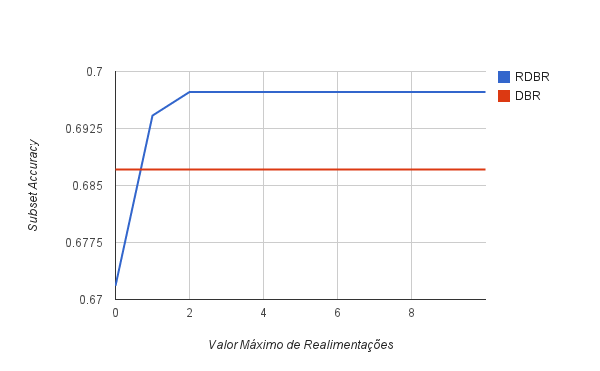
\includegraphics[width=1\textwidth] {Gmedicalj48_mrlm.png}
\end{figure}

\begin{figure}[h]
\label{fig:Gmrlm_2}
\caption{Gráficos do desempenho do \MRLMa~(eixo vertical) para vários valores máximos de realimentações (eixo horizontal)
representado nas linha azuis.
A linha em vermelha representa um limiar para o \MRLMa~cujo valor é o desempenho do DBR.}
\centering
% 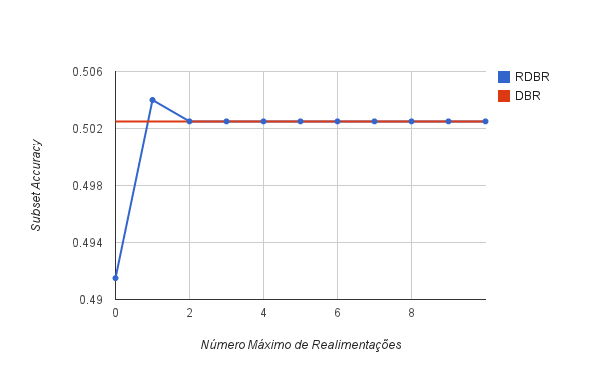
\includegraphics[width=1\textwidth] {Gbirdsj48_mrlm.png}
% 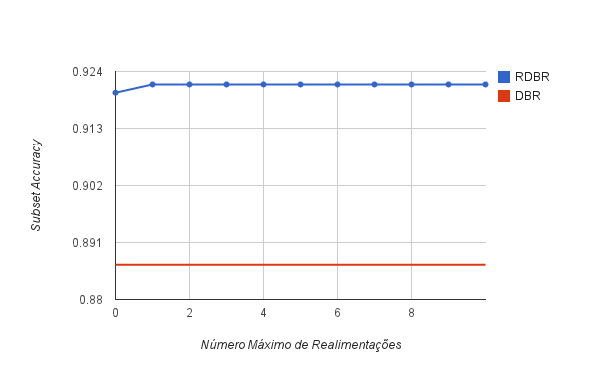
\includegraphics[width=1\textwidth] {Ggenbaseknn_mrlm.png}
\end{figure}



É importante analisar o quanto o método aumenta o tamanho da base de dados uma vez que isso acarreta no aumento
do tempo de execução do algoritmo. Sendo $l$ o número de rótulos, $n$ o número de instâncias de treino
e $m$ o número de atributos da base original, na fase de treinamento do \MRLMa, o número de base de dados utilizadas são
$2l$, cada uma contendo $n$ instâncias. Em metade delas, as instâncias contidas tem $m$ atributos e na outra metade $m+l$ atributos.
Já na fase de predição do algoritmo, no pior caso, o algoritmo usa $(r+1)l$ bases de dados de $n$ instâncias onde na primeira base, o
número de atributos é igual a $m$ e nas restantes é igual $m+l$. Vale ressaltar que nem todas essas bases de dados são
armazenados explicitamente na mémoria em espaços diferentes, algumas são reutilizadas no processo de predição.

% Em relação a complexidade algorítma do \MRLMa, ela pode ser
% aproximada pelo número de atributos destinados ao classificador base, uma vez que é um método de transfomação
% e a maior parte do custo computacional se encontra no classificador base.
% A complexidade 




\chapter{Avaliação e Análise Experimental}
\section{Método de Comparação}
\label{sec:methodcomp}

A comparação e estudo dos métodos é feita considerando o custo computacional e a qualidade de predição.
A qualidade de predição é estimada pelo método de avaliação por validação cruzada \ref{sec:modelav} com 10 grupos
(\textit{10-fold cross-validation}) sobre as \Nbases~bases de dados, todas apresentadas pela tabela \ref{tab:datas}.
Todas as bases de dados foram obtidas de repositórios públicos pelo seguinte
endereço virtual ??.
Para quantificar a qualidade de predição, foram escolhidas as seguintes métricas:
% Hamming Loss, Accuracy, Subset Accuracy, Ranking Loss, ...@@@.

% As métrica escolhidas e os motivos pela qual foram escolhidas são os seguintes:
\begin{itemize}
 \item Subset Accuracy, pois é rígida @@@ etc...
 \item @@@
 \item @@@
 \item Tempo computacional, pois é @@@ etc...
\end{itemize}

As fórmulas para o cálculo de cada uma das métricas são apresentadas na seção \ref{sec:metrics}.
É interessante mostrar os resultados experimentais usando diferentes métricas, pois cada uma captura
um aspecto diferente da classificação.

Este capítulo se encontra dividido em duas seções, na primeira foram analisados os
resultados dos métodos de transfomação para cada classificador base.
Já na segunda seção cada combinação de método multirrótulo com classificador base foi considerado
um método de transformação e seus resultados são comparados entre si juntamente com os métodos multirrótulos
de adaptação.
Num total, foram utilizados \Nml~\MML, \NmlT~da categoria de transformação e \NmlA~de adaptação: ??


\section{Classificadores Bases}
Nesta seção, são apresentados várias tabelas dos experimentos citados na seção anterior.
Para cada tabela é apresentado os resultados métricos de todos os métodos multirrótulo quando aplicados para
com um único classificador base. Em cada uma é analisado qual método multirrótulo combina melhor com o classificador
base escolhido. Em todas as tabelas o valor em negrito
representa o melhor valor obtido dentre os métodos multirótulos. 	


% No entanto, uma vez que é impossível obter uma única ordenação dos métodos
% usando múltiplos critérios,
% optou-se por usar a média dos ranking das métricas como
% o único critério de ordenação ao levantar pontos conclusivos sobre os métodos. 




% A comparação é antecedida por um estudo dos parâmetros dos métodos
% cujo objetivo principal é encontrar os parâmetros que devem ser usadas na comparação dos métodos. Objetivos secundários são
% espeficicados nas seções \ref{sec:study1} e \ref{sec:study2}, especialmente dedicadas para esse estudo.
% O objetivo principal é alcançado ao analisar a alteração do comportamento dos métodos quando seus parâmetros são alterados.
% O estudo dos parâmetros foi dividido em dois subestudos:
% \begin{enumerate}
%  \item estudo individual, que tem por objetivo analisar os parâmetros únicos de cada método individualmente.
%   \item estudo de grupo, que tem por objetivo analisar os parâmetros que são idênticos para um grupo de métodos.
%   Nesse caso o parâmetro que representa a escolha do classificador binário base para os método baseados em transformação é
%   analisado. 
% \end{enumerate}
% 
% O estudo de grupo tem como objetivo principal descobrir a melhor forma de comparar esses métodos entre si e
% entre outros métodos, por exemplo, compara-los usando o mesmo parâmetro em cada um ou compara-los usando o melhor parâmetro
% de cada um.
% 
% 
%   Para mais detalhes sobre os motivos desse estudo bem como seus resultados e conclusões na seção \ref{sec:study1}.
  
% 
% \section{Estudo dos Métodos baseados em Transformação}
% \label{sec:study1}
% \begin{verbatim}
%  -Listar métodos.
%  -Falar como vai ser comparado cada método (teste estatístico, rankeamento, métrica boa) para comprovar a hipotese.
%  -Apresentar resultados. (experimentos,tabela, gráficos...)
%  -Conclusão sobre os resultados
% \end{verbatim}
% 
% Nessa seção os \NmlT~\MMLs~de transformação são estudados com relação a suas qualidades. (@@@ listar os métodos de transfomação.)
% A escolha do classificador base para cada um dos métodos foi reestrito para \Ncb~classificadores: @@@.
% Esse subestudo tem como objetivo principal encontrar os classificadores $c_1^*,c_2^*,c_3^*,c_4^*,c_5^*$ que serão utilizados pelos
% métodos $T_1,T_2,T_3,T_4,T_5$.
% Para isso, analisou-se duas características:
%   \begin{enumerate}
%   
%   \item a variação do ranking do método segundo um critério de qualidade ao variar o classificador base
%   para uma base específica.
%   \item a variação do ranking do classificador base segundo um critério de qualidade ao variar o método multirrotulo.
%   \end{enumerate}
% 
% A comparação é realizada pelo rankeamento dos métodos, ou seja, os \MMLs~de transformação são submetidos a testes experimentais
% e ordenados segundo seus desempenhos de tal forma que para cada métrica e classificador base,
% é atribuído ao \MML~um valor correspondente a sua ordem, entre 1 e \NmlT. A ordenação por uma métrica
% é independente da ordenação da outra. 
% Os resultados experimentais são apresentados nas tabelas \ref{tab:study1-R-emotions},\ref{tab:study1-R-birds},..., uma para cada base de dados utilizada.
% Por essas tabelas, já podemos observar as duas características desejadas, enumeradas anteriormente na seção \ref{sec:methodcomp},
% mas para facilitar, construiu-se também as tabelas \ref{tab:study1-resumo}, que são resumos das tabelas ???.






\chapter{Conclusão}